\documentclass{llncs}
%
\usepackage{makeidx}
\usepackage{graphicx}
\usepackage{mwe}
\usepackage{subfig}
%
\begin{document}
%
\frontmatter
%
\pagestyle{headings}
\addtocmark{Augmented Ultrasound}
\title{Ultrasound Augmentation: Rapid 3-D Scanning for Tracking and On Body Display}
\titlerunning{Ultrasound Augmentation}
\author{Maeliss Jallais \and Hastings Greer \and Stephen Aylward}
\institute{Kitware Inc, Carrboro NC 27510, USA}
%
\mainmatter
\maketitle

\begin{abstract}
By using a laser projector and high speed camera, we can add three capabilities to an ultrasound system: tracking the probe, tracking the patient, and projecting information onto the probe and patient. We can use these capabilities to guide an untrained operator to take high quality, well framed ultrasound images which can be passed to existing or novel diagnosis algorithms
\end{abstract}


\section{Motivation}
We have developed algorithms that analyze ultrasound signals to detect internal bleeding. [3] These algorithms are part of a point-of-care, computer-assisted ultrasound system that is intended to aid in the triage of patients with abdominal trauma at the scene of an accident, helping emergency medical service (EMS) personnel save lives by assisting them in deciding when to order expedited transport and initiate life-saving measures in the field.

The remaining challenge with deploying our point-of-care, computer-assisted ultrasound system is, even though internal bleeding can be automatically detected, the EMS personnel must know where to place and how to manipulate an ultrasound probe at various anatomic locations in order to thoroughly examine the regions of the abdomen where blood tends to pool. Additionally, the EMS personnel must ensure that high-quality ultrasound data is being acquired. These positioning and data-quality-assessment tasks require extensive anatomic and ultrasound training—beyond what most clinicians and/or EMS personnel typically receive.

To solve this problem, we are investigating a variety of methods and user interfaces to guide EMS personnel in probe placement, to inform them of data quality and to produce diagnoses. One innovative method that we are exploring involves the combination of  patient and probe tracking with augmented reality to create an “augmented ultrasound” system.

\section{Augmented Ultrasound}
Rather than displaying data and instructions on a screen, our augmented ultrasound system proposes to concisely convey guidance and diagnoses by projecting instructions onto the surface of the patient. There are several advantages. Unlike a screen, a projection does not require the operator to look away from the patient. In addition, when combined with a tracker, the projection can provide directions in absolute terms. For example, our system will be able to direct the operator to “Place the scanner on the bullseye,” instead of relying on more abstract instructions such as “Place the scanner on the right side of the patient’s chest, half-way between the nipple and the shoulder.” Furthermore, instructions can be updated based on the tracked movement of the ultrasound probe and the images/anatomy captured in the ultrasound data, ensuring coverage of an anatomic area or flashing a warning icon when the probe is not making sufficient contact with the skin.

To operate, the augmented ultrasound system must be able to track an ultrasound probe and the surface of the patient’s body and then use the generated model of the body and the position of the probe to accurately project graphics/instructions onto the patient’s body.  Furthermore, the augmented ultrasound system must work in sunlight and in rugged environments with minimal set-up time so that it can be applied at the scene of an accident.  

In the next section, we discuss how we formed a three-dimensional (3D) model of a scene using a laser projector and a high-speed camera. Then, we describe how we track objects in that scene.

\section{3D Scene Modeling}
To form a 3D model of a scene, we replicated and extended the work in a paper by researchers at Carnegie Mellon University that involved a structured light 3D scanner based on a portable projector, which uses laser projection technology, and a high-speed camera. (See Fig. 1, adapted from [1].) The laser projector draws only one line of a projected image at a time, but it does so fast enough to enable the human eye to see the entire image. The high-speed camera is capable of precise timing and fast shutter speed. These properties allow the camera to take a picture as the projector draws a specific line of the image. Through a one-time calibration of the camera and the projector, and through using structured-light reconstruction algorithms, each point on a projected line can be efficiently and accurately triangulated to a point in 3D space (i.e., each illuminated point seen in a camera image is at the intersection of the plane/line of light emitted by the projector and the corresponding pixel/line viewed by the camera). The camera/projector calibration process is adapted from the method developed at Brown University [2], which is based on OpenCV and uses the camera application programming interface (API).
\begin{figure}
\centering
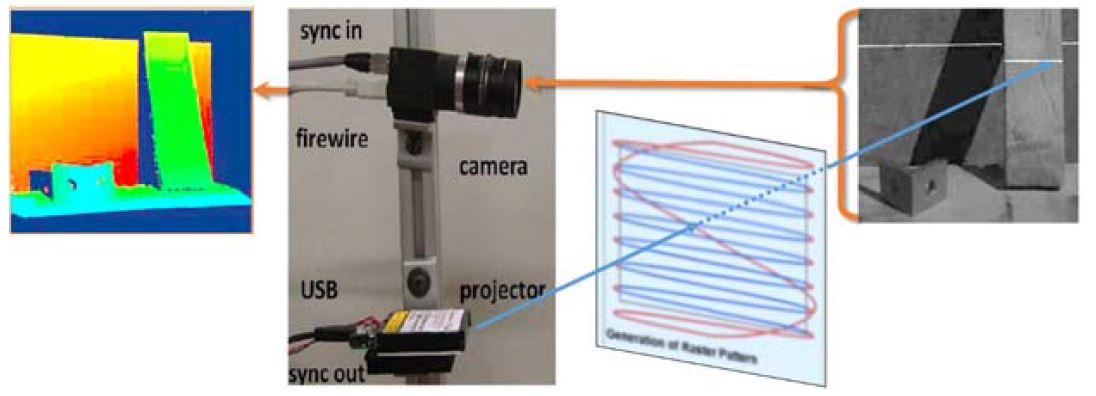
\includegraphics[width=10cm,height=10cm,keepaspectratio]{plan}
\caption{
The augmented reality system uses a pico projector (based on laser projection technology) to display an image in a scene. A high-speed camera sees the individual lines being drawn by the projector to create the image. Via appropriate camera calibration, custom circuitry to detect the vertical reset of the laser and depth from structured lighting algorithms, a 3D model of the scene can be formed at very high resolution in about one second.
}
\end{figure}

Our system is composed of a Grasshopper3 camera and a SONY mobile projector MP CL1. With a resolution of 2048 x 1536, we can use the camera at a frame rate of 300 fps. The update rate per image of the laser projector is 60Hz in scan line order. Given its resolution of 1920 x 720, it projects 43,200 lines/s.

The augmented ultrasound system works under varied lighting conditions for three reasons. First, the shutter speed simplifies the detection of which pixels are illuminated by the projector. It suppresses ambient light, even direct sunlight, simply by remaining open for no more than a tiny fraction of a second.

\begin{figure}
\centering
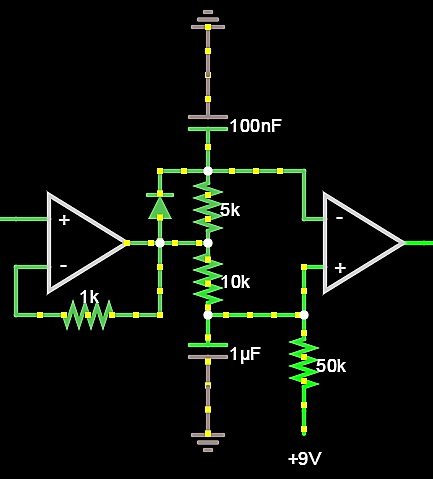
\includegraphics[width=10cm,height=10cm,keepaspectratio]{circuit}
\caption{
Circuit diagram of the photo detector system used to determine when the laser returns to the upper left and begins drawing a new image (approximately every 1/60th of a second).
}
\end{figure}
This benefit arises because the laser projector illuminates each point very brightly, but only for a fraction of a millisecond. Alternatively, ambient sources like the sun illuminate continuously at a lower intensity. Second, we use background subtraction to further reduce the effect of ambient light. In particular, from each image that is taken, we subtract an image from when the laser is in a different location.  Third, we apply a custom method that quickly detects the brightest point on a vertical scan line in a grayscale image.

The most difficult challenge with our low-cost, compact ultrasound augmentation system was that the horizontal sync signal produced by the projector/HDMI protocol was not phase-locked to the actual vertical movement of the laser. For this reason, we opted to trigger the camera off the light emitted by the projector, using a photocell and a pair of Operational Amplifiers.  See Fig. 2.

Sample results from the system are shown in Fig. 3.  We are now optimizing the system for speed by expanding upon the trigger mode on the camera to capture up to three lines from each frame (i.e., every time the laser sweeps the scene).

\begin{figure}[h]
\centering
\subfloat[]{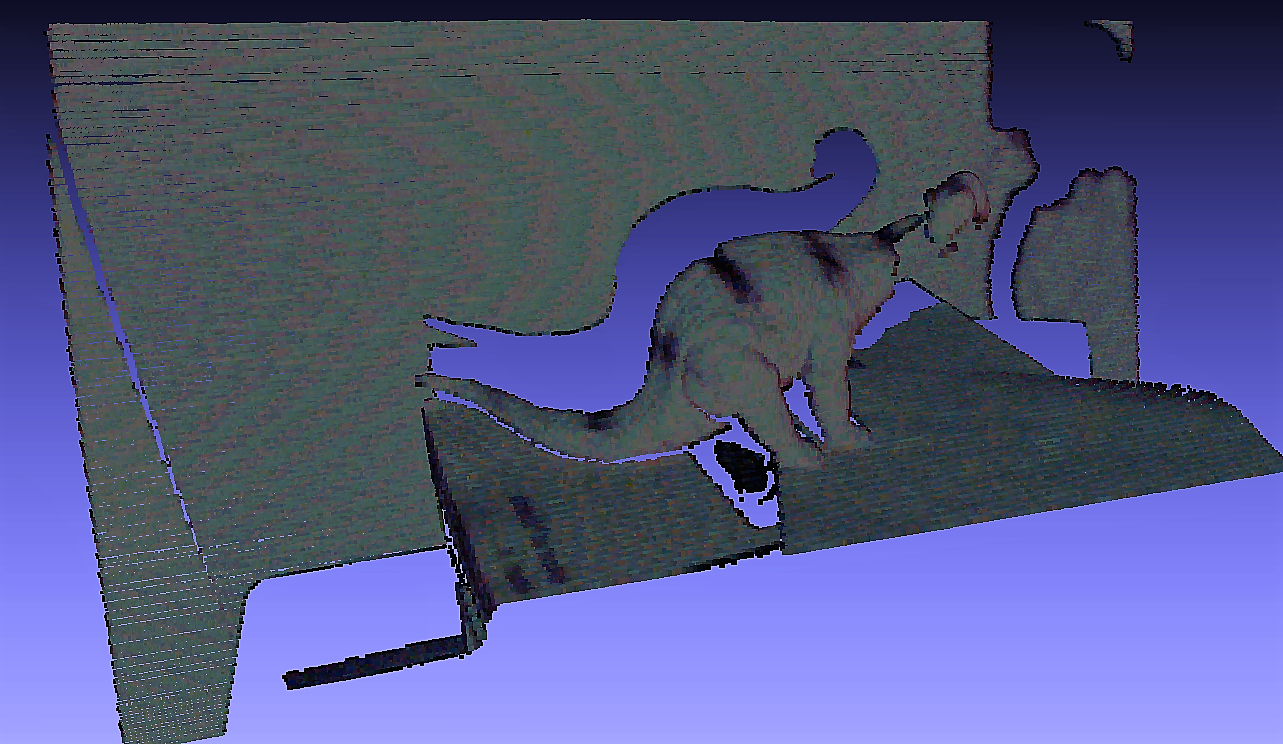
\includegraphics[scale=.14,keepaspectratio]{dino}}\hfill%
\subfloat[]{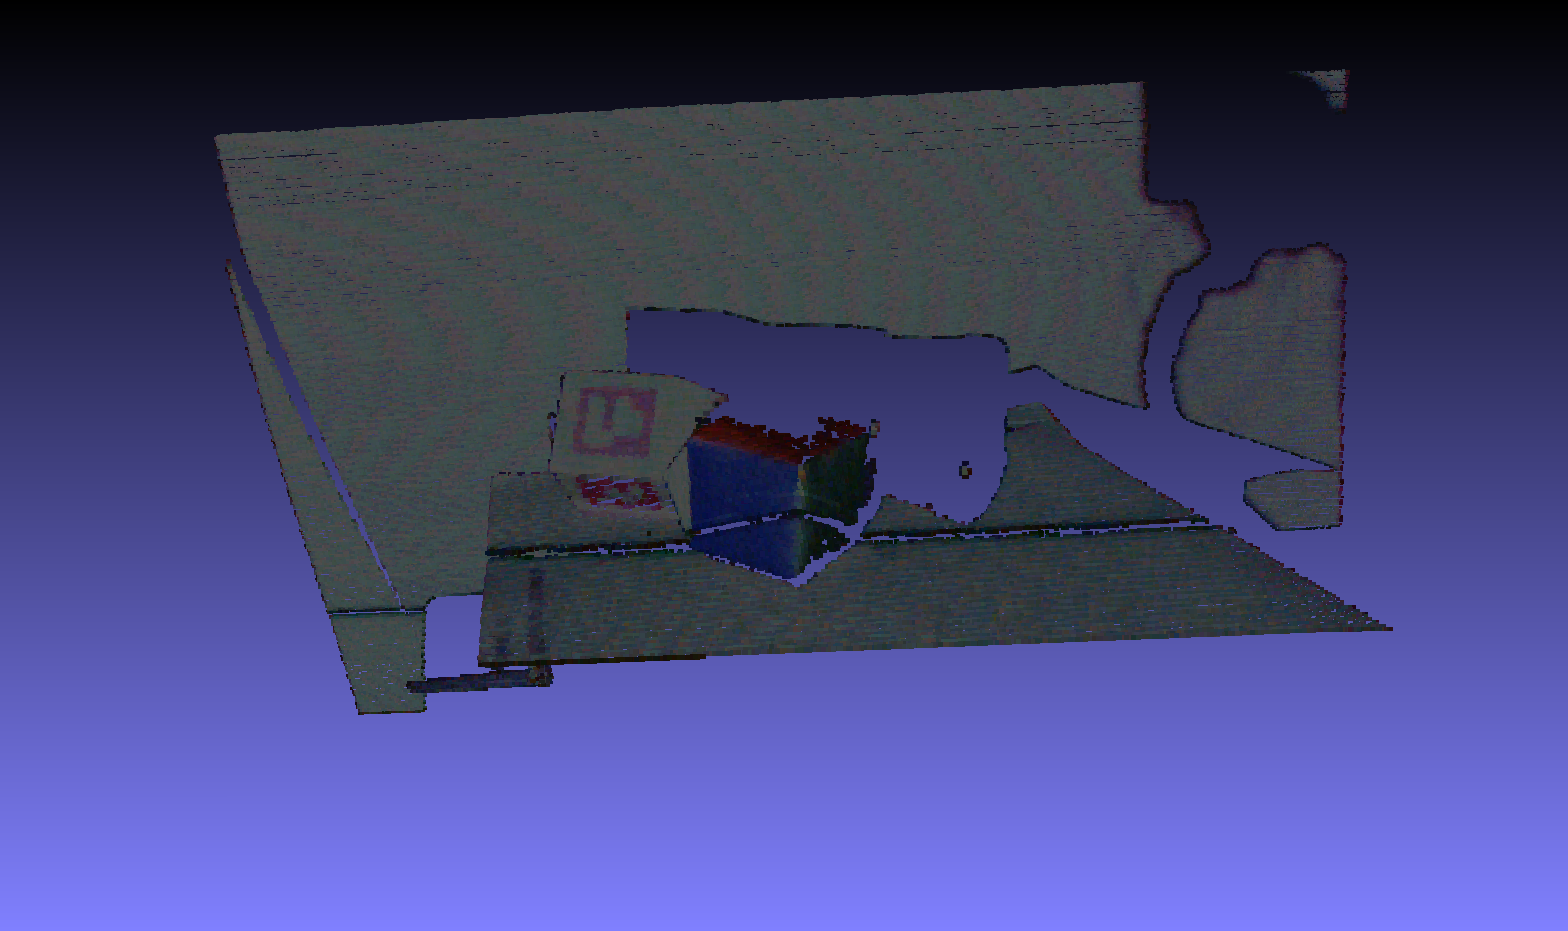
\includegraphics[scale=.14,keepaspectratio]{block}}\\
\subfloat[]{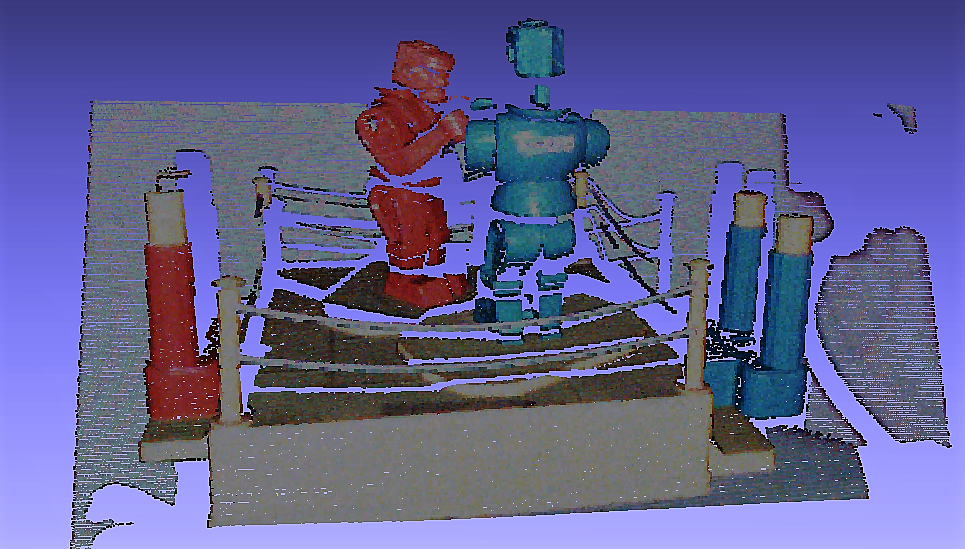
\includegraphics[scale=.14,keepaspectratio]{rockem}}
\caption{
Examples of 3D scenes captured by our system.
}
\end{figure}

\section{Object Tracking}
Having formed a 3D model of a scene, the next step in ultrasound augmentation is to track an ultrasound probe. To that end, we mounted a multi-cubed, color-tagged marker (designed by InnerOptic) on the probe.  The colors of the cube are red, blue and green. They are optimized for the response curves of the color detectors in the camera. By determining the intersection of three adjacent faces on the cubes, we can determine the position and the orientation of the ultrasound probe.

To simplify and speed the tracking algorithm, instead of estimating the specific location of each cube face, we estimate the planes that contain each of the faces of the cube and then solve for the intersection of those planes. The plane detection method begins with color pixel detection, using statistical models of the appearance of the cube faces under a range of lighting conditions. Depending on the image from the projector, the ambient light and the adjacent objects in the environment, extraneous pixels may be incorrectly identified as cube pixels based on color alone. To eliminate extraneous pixels, we compute the gravity centers for each target color using robust statistics. Knowing the expected position of each face relative to the others, we can redefine the estimates of the centers of gravity by eliminating colored pixels that are inconsistent with the expected relative positions of each face and too far from the estimated centers of gravity. To further reduce the influence of extraneous pixels, we also estimate the equations of the planes using the random sample consensus (RANSAC) algorithm. It randomly picks three points, computes the plane defined by them and then scores that plane based on how many other cube points are included in that plane. Ultimately, the planes with the best scores are chosen. The intersection point of the three chosen planes is then used to define the position and the orientation of the probe in space. A sample result of three detected planes intersecting the scene is shown in Fig. 4.

\begin{figure}
\centering
\begin{tabular}{cc}
\centering
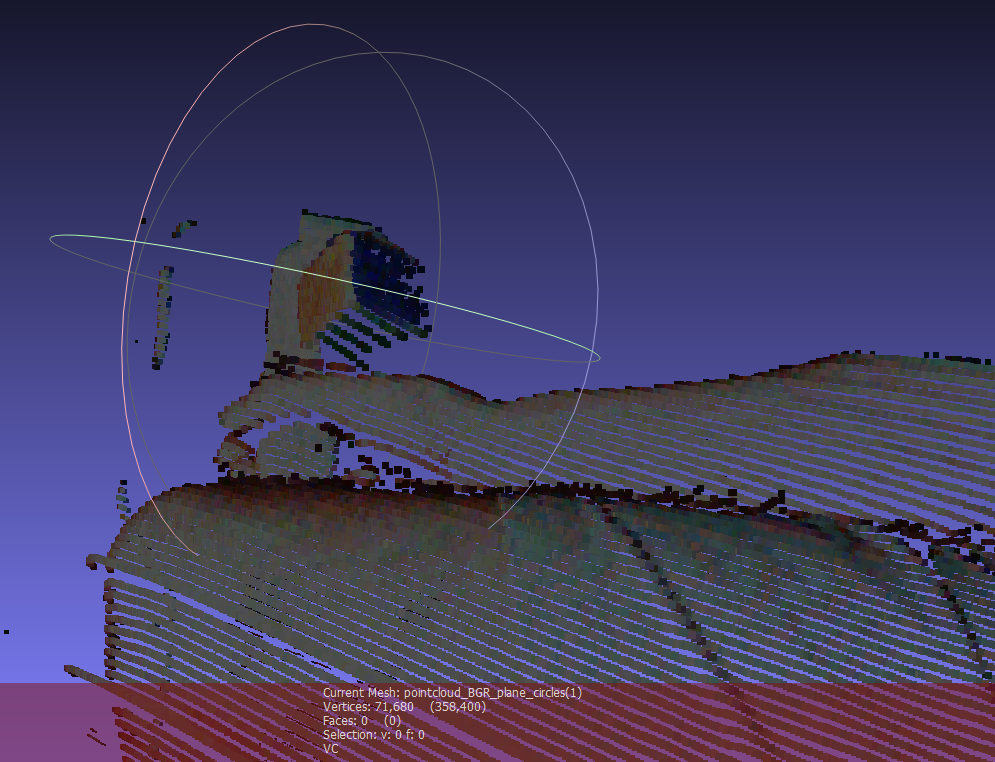
\includegraphics[scale=.233]{linesNotFound} &
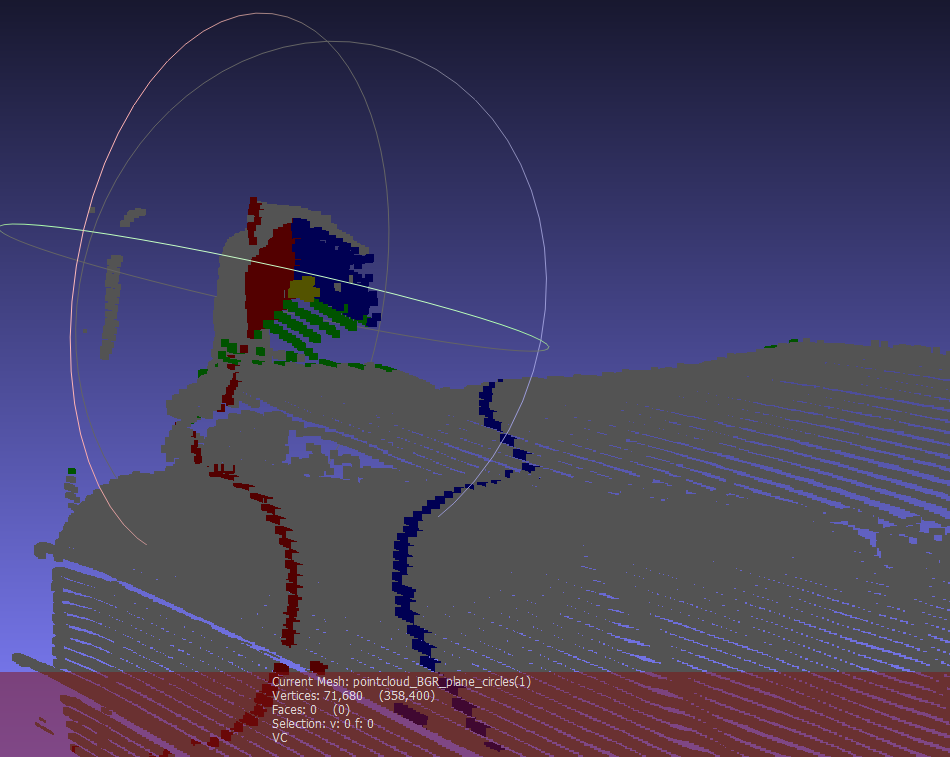
\includegraphics[scale=.233]{linesPointcloud}\\
(a) & (b)
\end{tabular}

\caption{
(a) The raw point cloud before cube detection, (b) The collected point cloud is shown in white. The intersection of the estimated red, green and blue planes with that point cloud are shown. This indicates that the faces of the cube are well represented by the estimated planes.
}
\end{figure}

\section{Projecting onto the Scene}

Once a point cloud is captured and the probe is located, the system must project information onto surfaces int he scene. Our approach takes advantage of an unusual property of our scanner: that it can trade off between point cloud density and frame rate. A very high density point cloud is captured as the system is initialized, and updated as needed if the patient moves, for use in reprojection. Coloring operations, such as drawing circles, lines, images, or text, are applied to this high resolution point cloud. This allows positions and orientations of text to be manipulated in 3-D, 1 to 1 scale coordinates. Each relevant point is then colored by tracing a ray through it into the virtual image. Finally, the high resolution pointcloud is transformed by "camera matrix" of the projector, and drawn to a bitmap, which is displayed through the projector. 

\section{Conclusion}
Ongoing work focuses on quantifying the performance of this algorithm.  Current studies indicate 2mm consistency within a 30cm x 60cm x 60cm operating environment.  The system has been shown to be insensitive to a wide range of ambient light brightness and to the image being projected into the scene.

The probe tracker data will be used, in combination with a custom image reconstruction technique, to compound a sequence of imprecisely and sparsely tracked ultrasound images into a complete 3D Volume.

First, the volume and pointcloud will be analyzed for image suitability. If the image is not suitable for the diagnosis requested by the EMS, information on how to improve the image will be projected directly onto the patient or probe, such as: 
Lateral adjustements of the probe,
angle adjustment of the probe
application of ultrasound gel
increase or decrease in probe pressure.

Once the system is satisfied with the image quality, This volume will be automatically analyzed by domain specific algorithms that produce information needed by EMS, such as vein position and patency, presence of pneumothorax, or presence of abdominal bleeding. Information such as abdominal bleeding or pneumothorax can be presented on a traditional screen or via audio. Vein position can be presented as color projected directly onto the skin above the vein.

The final system is illustrated in Fig. 5.  The figure depicts the system indicating where a needle should be inserted for peripheral vascular access with ultrasound guidance.

\begin{figure}
\centering
\begin{tabular}{cc}
\centering
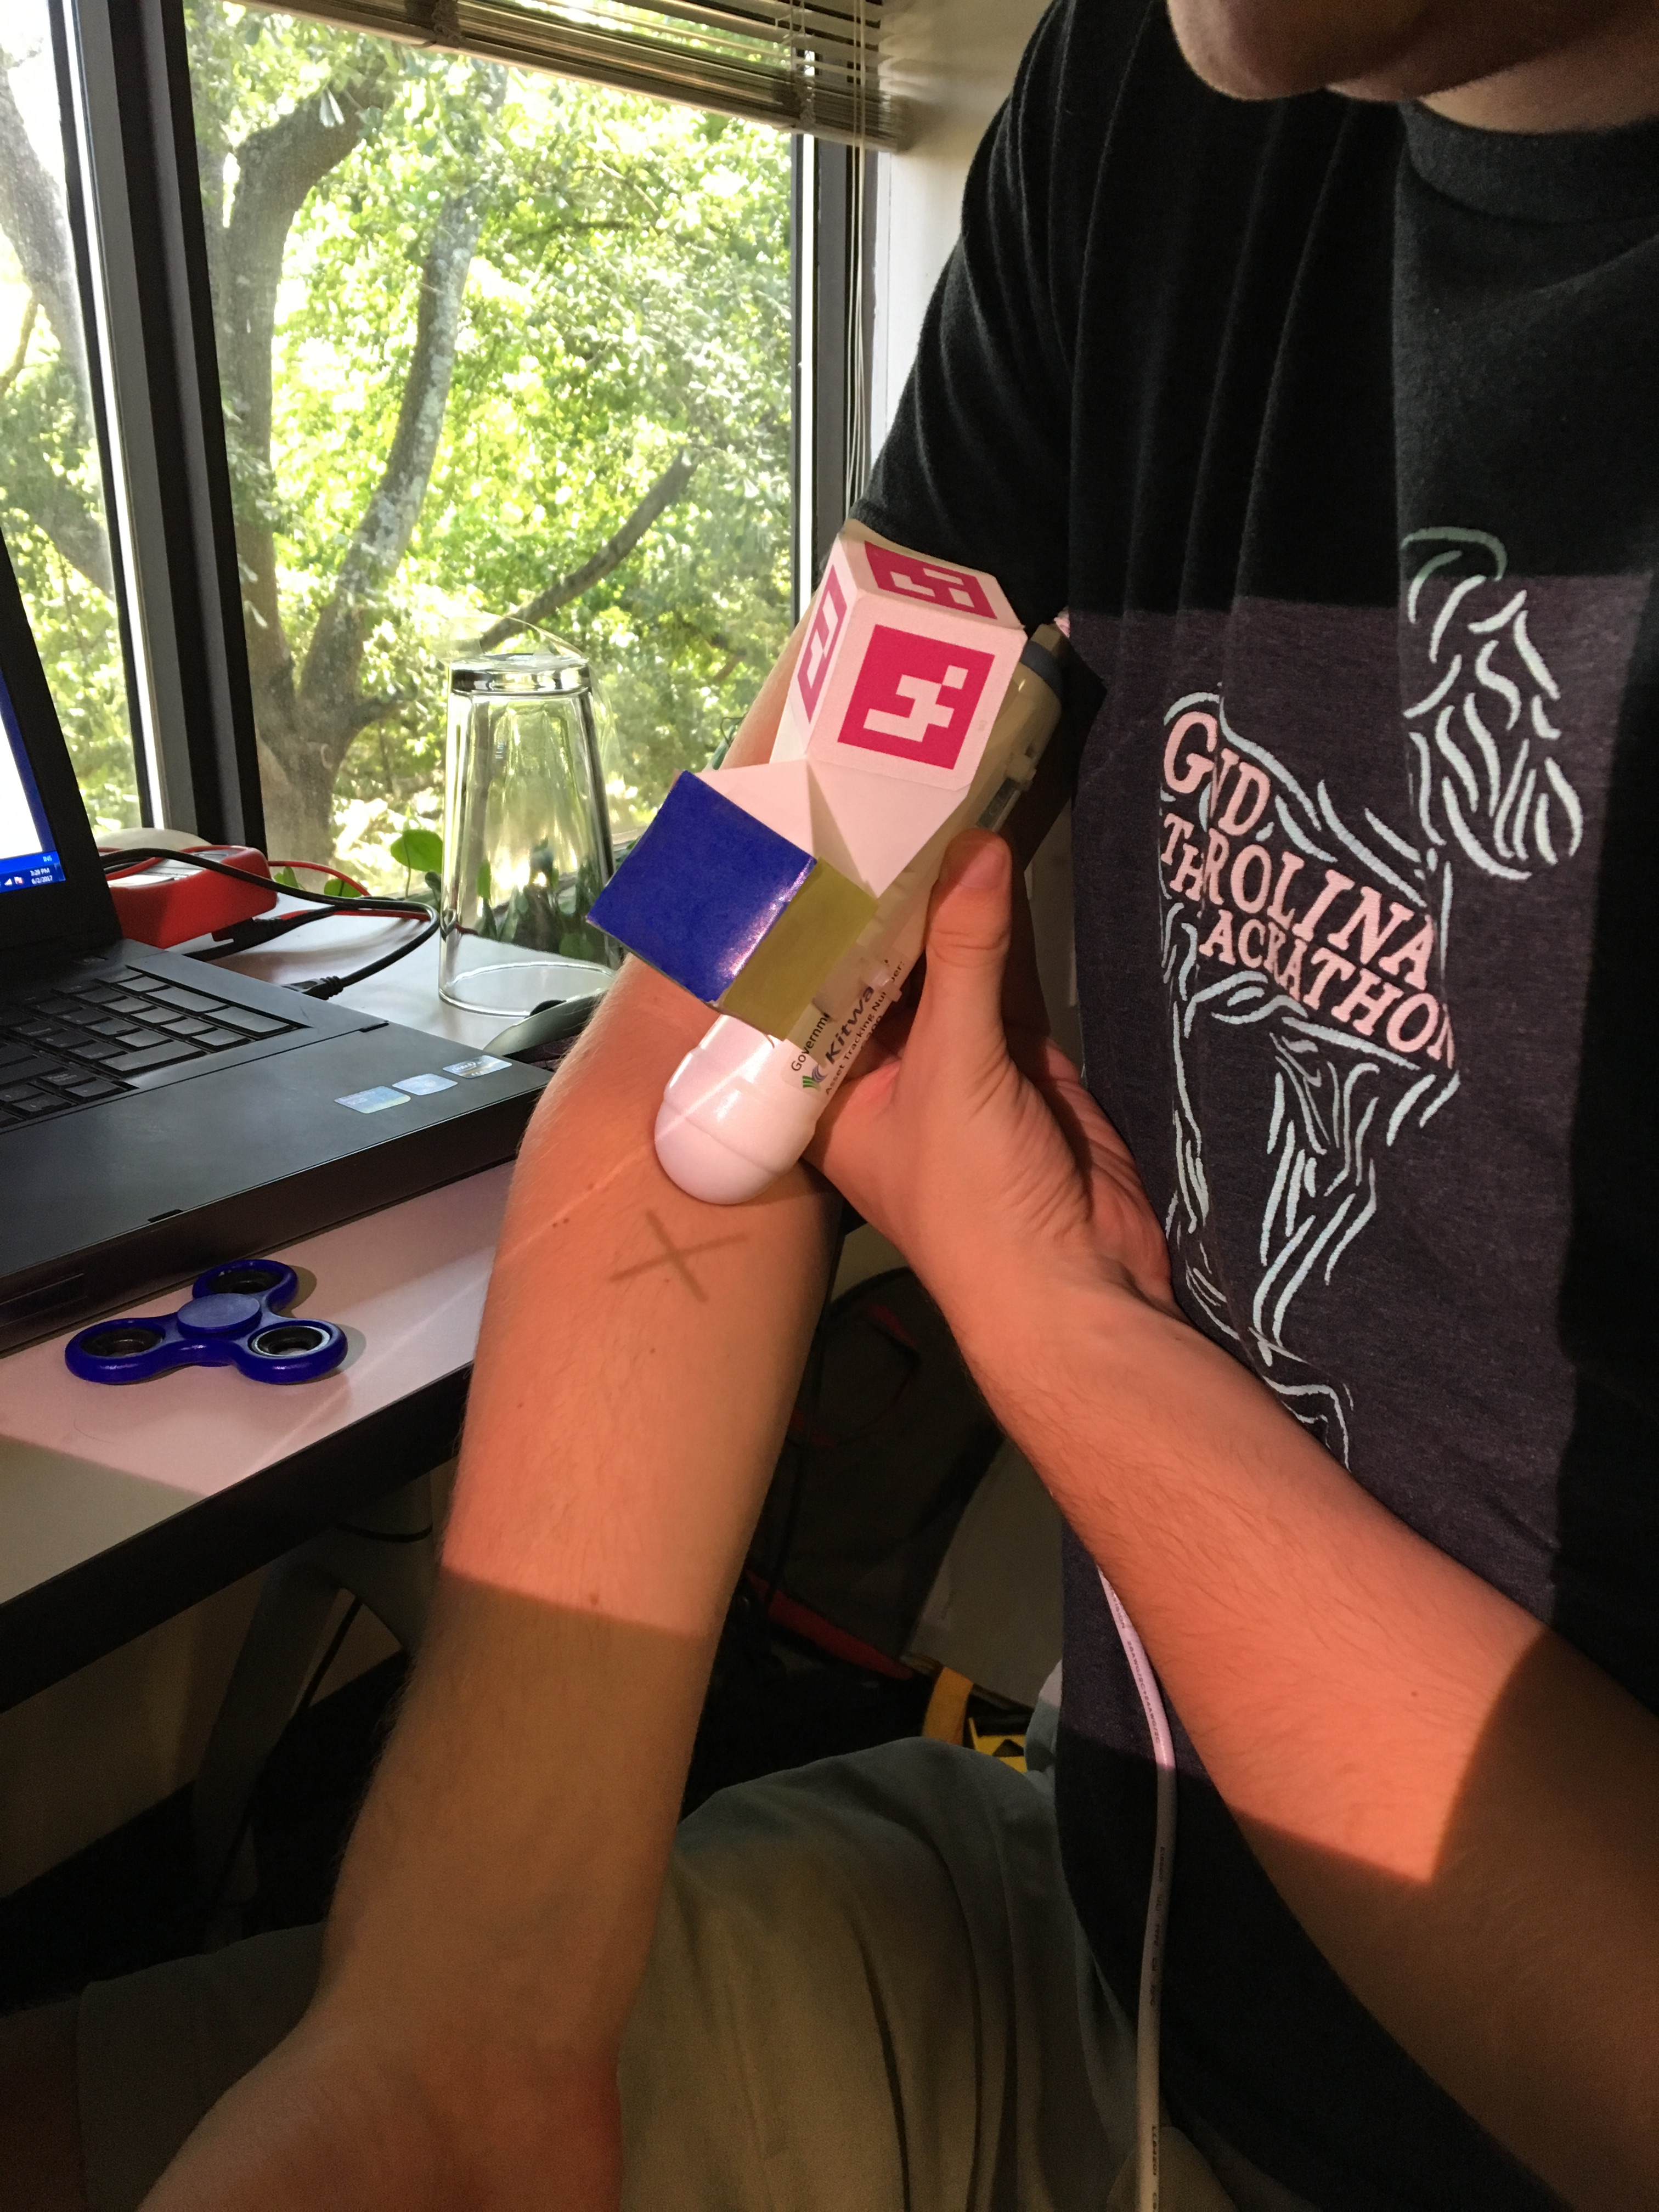
\includegraphics[height=5.5cm,keepaspectratio]{Hastings_arm} &
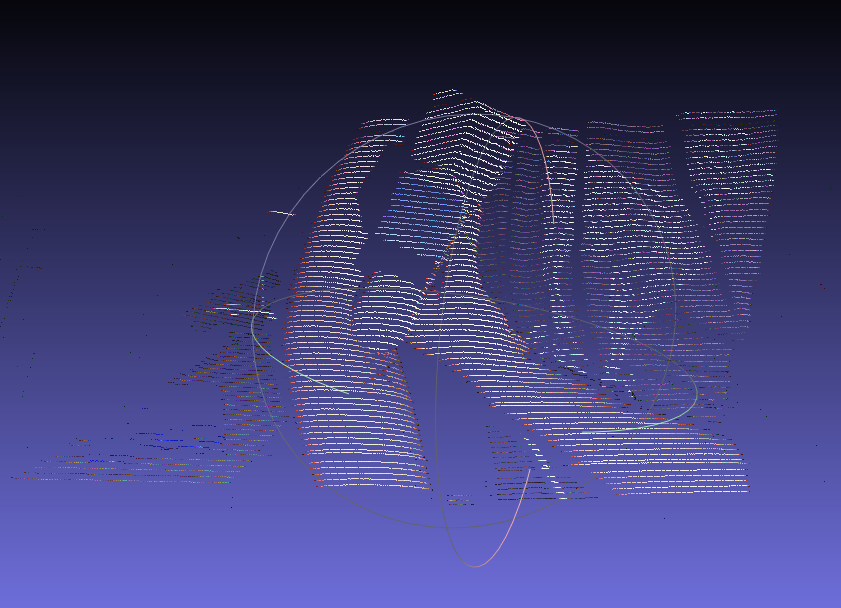
\includegraphics[height=5.5cm,keepaspectratio]{Hastings_arm_pointcloud}\\
\end{tabular}

\caption{An illustration of the end goal of the system. A target (black X) is projected onto the skin as the camera computes depth from structured light using the raster lines of the projected image as that image is drawn. Ultrasound can be used to detect peripheral vessels, select needle insertion locations and verify needle placement patency.
}

\end{figure}


\section*{Acknowledgments}
This work was funded, in part, by the following grants.

\begin{itemize}
	\item NIH/NIBIB: “In-field FAST procedure support and automation” (R43EB016621)
	\item NIH/NINDS: “Multimodality image-based assessment system for traumatic brain injury” (R44NS081792)
	\item NIH/NIGMS/NIBIB: “Slicer+PLUS: Collaborative, open-source software for ultrasound analysis” (R01EB021396)
\end{itemize}

%
% ---- Bibliography ----
%
\begin{thebibliography}{}
%
\bibitem[1]{1}
C.Mertz, S. J. Koppal, S. Sia, S.G. Narasimhan. A low powered structured light sensor for outdoor scene reconstruction and dominant material identification. In CVPRW IEEE, 2012.

\bibitem[2]{2}
D. Moreno, G. Taubin. Simple, Accurate, and Robust Projector-Camera Calibration

\bibitem[3]{3}
S. R. Aylward, M. McCormick, H. J. Kang, S. Razzaque, R. Kwitt, M. Niethammer. Ultrasound Spectroscopy

\end{thebibliography}


\end{document}

